\documentclass{article}

\usepackage{graphicx}
\usepackage{float}
\usepackage{geometry}
\geometry{
    top=0.5in,
    bottom=0.5in,
    left=0.5in,
    right=0.5in
}

% Document Information
\title{Demo 7: TimeQuest}
\author{Diego Lopez}
\date{\today}

\begin{document}
\maketitle

\begin{table}[h!]
    % \centering
    \begin{tabular}{ll}
        \textbf{Question 8.}
    \end{tabular}
\end{table}
\begin{table}[h!]
    \centering
    \begin{tabular}{|p{3cm}|p{3cm}|p{3cm}|}% \begin{tabular}{|c|c|c|}: Specifies a table with 3 columns, each centered (c). Vertical lines | separate the columns.
        \hline
         & Fmax & Setup Time \\ \hline
         Slow 1100mV 85C & 451.67 MHz & -19.472 \\ \hline % \\ \hline: Ends each row and adds a horizontal line.
         Slow 110mV 0C & 431.03 MHz & -20.359 \\ \hline
         Fast 1100mV 85C  & & -1.168 \\ \hline
         Fast 1100mV 0C & & -0.924 \\ \hline
    \end{tabular}
    \caption{No clock constraint}
\end{table}

\begin{figure}[htbp]
    \centering
    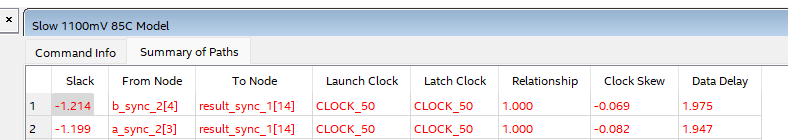
\includegraphics[width=0.8\textwidth]{PathSummary1.png}
    \caption{Path Summary}
    \label{fig:PathSummary1}
\end{figure}

\begin{table}[h!]
    \centering
    \begin{tabular}{ll}
        \textbf{Question 22.} & The clock was updated to match the results. \\
        \textbf{Question 23.} & The updated Fmax is now smaller than the Fmax without the constraint. This is becuase the smaller time constraint 
    \end{tabular}
\end{table}

\begin{table}[h!]
    \centering
    \begin{tabular}{|p{3cm}|p{3cm}|p{3cm}|}% \begin{tabular}{|c|c|c|}: Specifies a table with 3 columns, each centered (c). Vertical lines | separate the columns.
        \hline
         & Fmax & Setup Time \\ \hline
         Slow 1100mV 85C & 398.72 MHz & 0.000 \\ \hline % \\ \hline: Ends each row and adds a horizontal line.
         Slow 110mV 0C & 383.73 MHz & 0.000 \\ \hline
         Fast 1100mV 85C  & & 0.000 \\ \hline
         Fast 1100mV 0C & & 0.000 \\ \hline
    \end{tabular}
    \caption{With clock constraint}
\end{table}

\begin{figure}[!htbp]
    \centering
    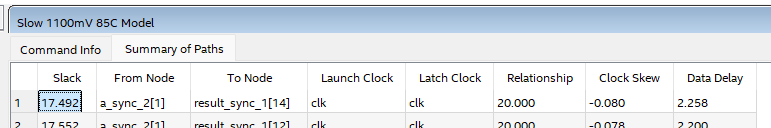
\includegraphics[width=0.8\textwidth]{PathSummary2.png}
    \caption{Path Summary for 100 paths}
    \label{fig:PathSummary2}
\end{figure}

\begin{figure}[H]
    \centering
    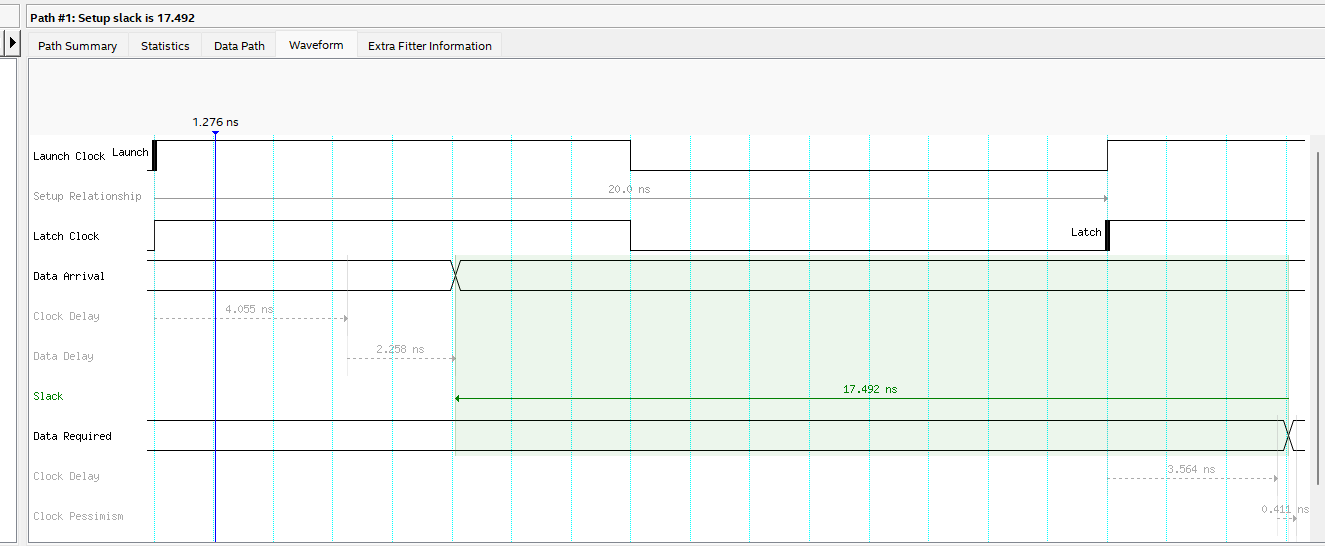
\includegraphics[width=0.8\textwidth]{PathWaveForm.png}
    \caption{Path Summary for 100 paths}
    \label{fig:Waveform}
\end{figure}

\section*{Conclusion}
\paragraph{TimeQuest is a timing analysis tool that helps test the timing of a design. The Fmax parameter is the max frequency and the Setup parameter is the minimum amount of time that the data must be stable before reaching a clock edge. Meeting the timing constraints ensures that the design operates reliably at the intended clock frequency, which is critical in embedded systems.}

\end{document}
